\documentclass[sigconf]{acmart}

\title{Climalytics AT}

\author{David Kalteis}
\email{s2410455001@fhooe.at}
\affiliation{\institution{FH Hagenberg}\department{Mobile Computing}\country{Austria}}

\author{Dominik Forsthuber}
\email{s2410455011@fhooe.at}
\affiliation{\institution{FH Hagenberg}\department{Mobile Computing}\country{Austria}}

\author{Michael Kerscher}
\email{s2410455014@fhooe.at}
\affiliation{\institution{FH Hagenberg}\department{Mobile Computing}\country{Austria}}

\begin{document}

\begin{abstract}
Your abstract here.
\end{abstract}

\maketitle

\section{Introduction}
Our project focuses on analyzing long-term weather trends and extreme climate patterns in Austria using scalable Big Data technologies. We aim to uncover patterns in temperature, precipitation, and extreme events across regions and over time.

\section{Dataset}
This dataset contains monthly aggregated climate data from various weather stations across Austria. Each entry includes numerous meteorological measurements (e.g., temperature extremes, precipitation, humidity, sunshine duration, frost days, wind data) over many years, making it suitable for large-scale time series and spatial weather analysis.
Time span: January 1970 – April 2025 (monthly resolution) \linebreak
The dataset used in this study was downloaded from GeoSphere Austria's climate data portal~\cite{geosphere_klima_v2_1m}.\\

\textbf{Downloaded datafiles:} 
\begin{itemize}
    \item \verb|climate_all_stations.csv    676 MB |
    \item \verb|parameter_metadata.csv       58 KB |
    \item \verb|stations_metadata.csv       168 KB |
\end{itemize}

\section{Research questions}
\subsection{How does the long-term trend in mean monthly temperature vary with elevation?}
\section{Long-Term Temperature Trends in High Alpine Regions (RQ1)}

\subsection*{Objective}
This research question investigates whether long-term temperature trends differ by elevation. To illustrate the phenomenon of elevation-dependent warming, this section focuses specifically on the highest elevation category: \textbf{2000+\,m (High Alpine)}. These zones are climatically sensitive and relevant for alpine climate analysis.

\subsection*{Methodology}
Using Apache Spark, monthly average temperature values (\texttt{tl\_mittel}) from the full dataset \texttt{climate\_all\_stations} were grouped by station and year. Elevation metadata was joined and used to classify each station into one of five predefined elevation bands.

To ensure focus and clarity, this analysis considers only the High Alpine category. The reasoning is threefold:
\begin{itemize}
    \item It is directly linked to climate vulnerability and snow cover dynamics.
    \item It exhibits strong and distinctive warming signals.
    \item It includes representative stations from multiple federal states.
\end{itemize}

Two additional plots were generated for context:
\begin{itemize}
    \item A distribution plot of all stations by elevation zone and region.
    \item A labeled diagram of the highest station per region to confirm extreme values.
\end{itemize}

\subsection*{Results and Interpretation}

\paragraph{Figure~\ref{fig:temptrend_highalpine}: Temperature Trends in the High Alpine Zone}
The line plot below shows annual average temperatures from 1970 to 2025 for each region in the High Alpine zone. A general increase is evident. While Tyrol and Vorarlberg exhibit consistent warming, Salzburg remains colder on average. Differences could be due to regional geography or data coverage.

\begin{figure}[htbp]
    \centering
    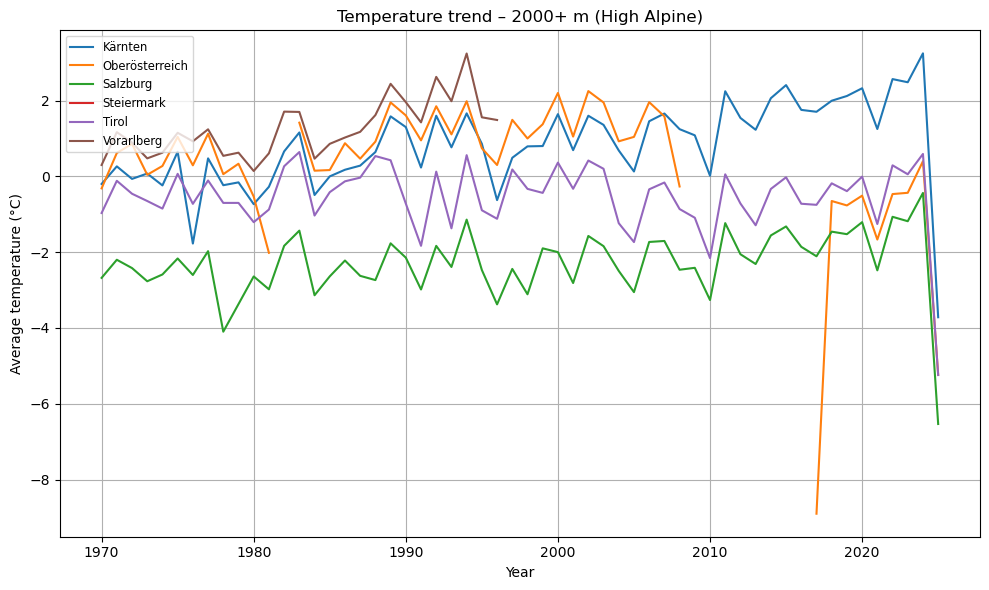
\includegraphics[width=\textwidth]{img/temptrend_highalpine.png}
    \caption{Average annual temperature trends (1970–2025) in 2000+\m High Alpine zone}
    \label{fig:temptrend_highalpine}
\end{figure}

\paragraph{Figure~\ref{fig:station_distribution_highalpine}: Altitude Distribution of High Alpine Stations}
This scatterplot validates that stations assigned to the High Alpine zone are located well above 2000+\m. The distribution also shows regional diversity, which supports cross-regional comparisons.

\begin{figure}[htbp]
    \centering
    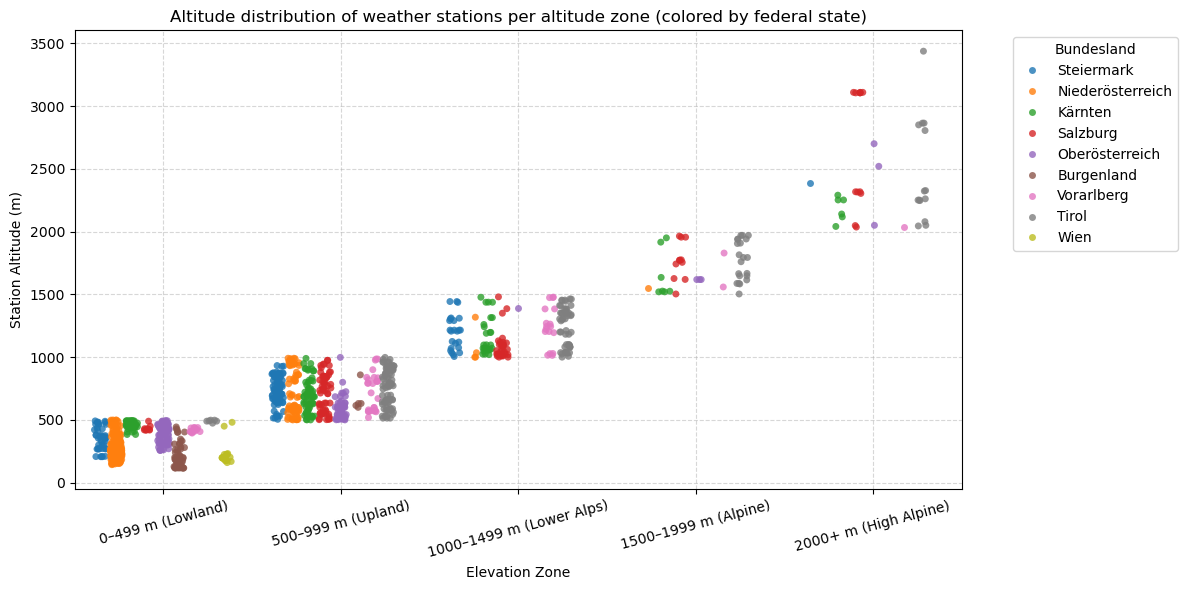
\includegraphics[width=\textwidth]{img/station_distribution_highalpine.png}
    \caption{Elevation distribution of stations by zone and region}
    \label{fig:station_distribution_highalpine}
\end{figure}

\paragraph{Figure~\ref{fig:highest_stations_labeled}: Highest Stations per Region}
This annotated plot confirms the locations and elevations of the highest weather stations per federal state. These are concentrated in Tyrol, Salzburg, and Carinthia—regions with substantial alpine terrain.

\begin{figure}[htbp]
    \centering
    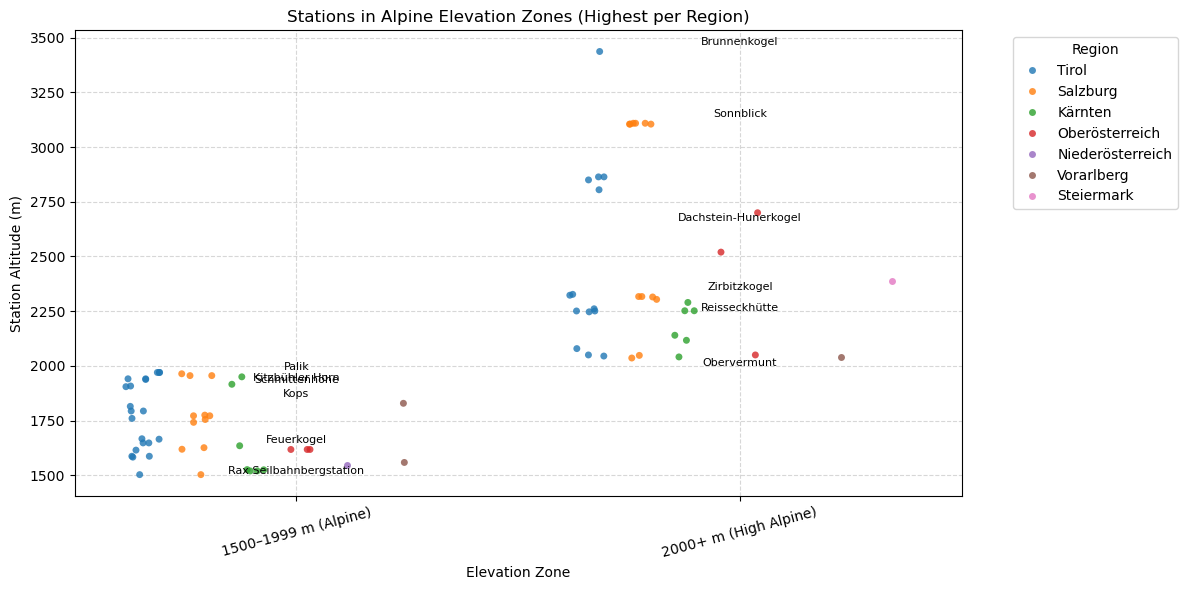
\includegraphics[width=\textwidth]{img/highest_stations_labeled.png}
    \caption{Highest station per region in Alpine zones with labels}
    \label{fig:highest_stations_labeled}
\end{figure}

\subsection*{Conclusion}
The High Alpine zone (2000+\m) in Austria shows a clear warming trend over the last five decades. Regional variation is present but does not detract from the overall pattern. By isolating a single elevation zone, this analysis enables focused insight while demonstrating elevation-dependent climate change.

The Spark-based implementation, which joins climate records with station metadata and performs grouped aggregations by year, proves efficient for scalable trend analysis. This framework can easily be extended to other elevation bands or regions.


\begin{figure}[H]
  \centering
  
\includegraphics[width=0.4\linewidth]{img/placeholder.png}
  \caption{Placeholder figure.}
  \label{fig:placeholder}
\end{figure}


\subsection{Which geographic zones (valleys, plateaus, alpine corridors) show the largest shifts in “hot days” (<= 30 C) and “frost days” (>= 0 C) since 1970?}
This question examines how the frequency of very hot days (>= 30 °C) and frost days (<= 0 °C) has changed since 1970 in three elevation‐based geographic zones:
\emph{valley} (<= 700 m), \emph{plateau} (701–1500 m), and \emph{alpine} (> 1500 m).

\subsubsection{Data Processing}
\begin{enumerate}
  \item \textbf{Load and transform:} Raw CSV data were ingested into a Spark DataFrame, with parsing of the “date” field and extraction of \texttt{year} for each station.
  \item \textbf{Parquet conversion:} The joined DataFrame (including elevation and zone labels) was repartitioned by \texttt{year} and \texttt{zone} and written to Parquet for efficient subsequent queries.
\end{enumerate}

\subsubsection{Data Analysis}
\paragraph{Full Time Series.}
We computed the annual, per‐station average counts of hot days (see Figure~\ref{fig:full_time_series_hot}) and frost days (see Figure~\ref{fig:full_time_series_frost}) for each zone.
\begin{figure}[ht]
  \centering
    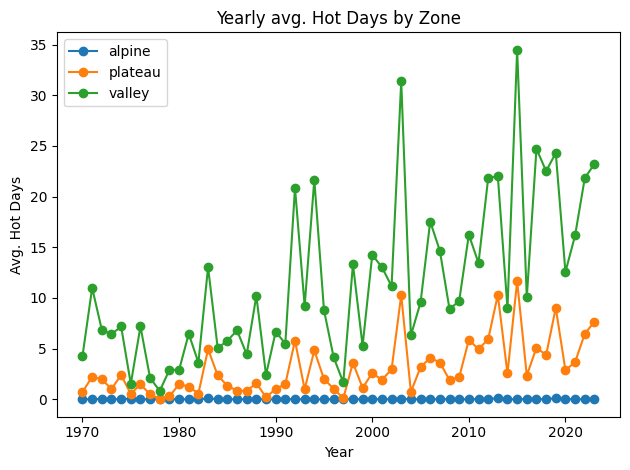
\includegraphics[width=0.45\textwidth]{img/full_time_series_hot.png}
  \caption{Yearly average hot‐day counts per station, by zone (1970–2023).}
  \label{fig:full_time_series_hot}
\end{figure}
\begin{figure}[ht]
  \centering
    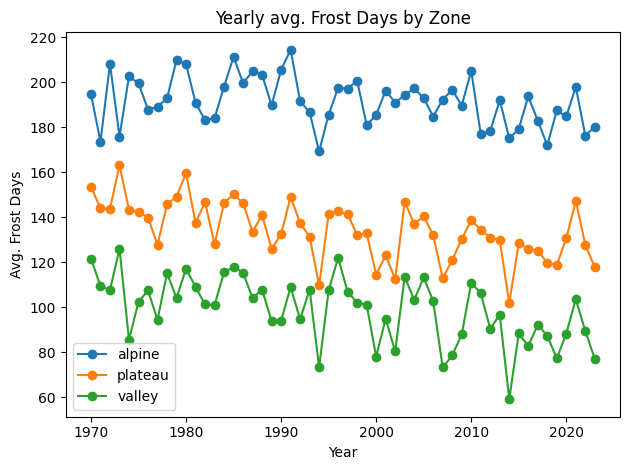
\includegraphics[width=0.45\textwidth]{img/full_time_series_frost.png}
  \caption{Yearly average frost‐day counts per station, by zone (1970–2023).}
  \label{fig:full_time_series_frost}
\end{figure}

\paragraph{End–Minus–Start Difference.}
To highlight net shifts, we compared the mean of 2014–23 vs.\ 1970–79 per zone, yielding the change in average hot‐ and frost‐days (see Figure~\ref{fig:decade_difference}).
\begin{figure}[ht]
  \centering
    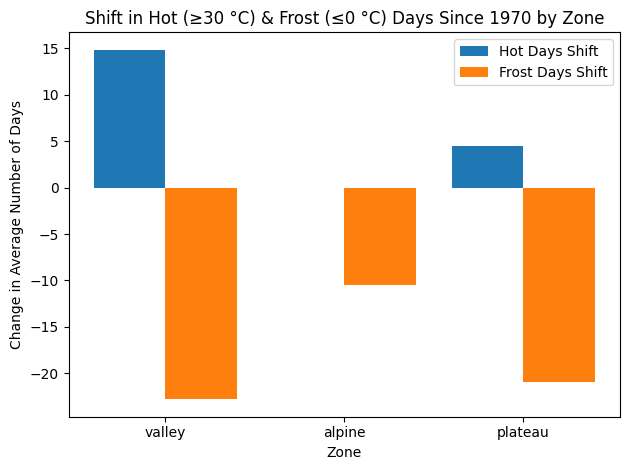
\includegraphics[width=0.45\textwidth]{img/end-minus-start_diff.png}
  \caption{Change in average hot and frost days (2014–23 minus 1970–79) by zone.}
  \label{fig:decade_difference}
\end{figure}

\paragraph{Linear Regression Trend.}
Finally, we fitted a simple linear model (OLS) of day‐count vs.\ year for each zone, extracting the slope (days per year), $R^2$, and $p$–value to quantify rate and significance of change (see Figure~\ref{fig:linear_trend}).
\begin{figure}[ht]
  \centering
    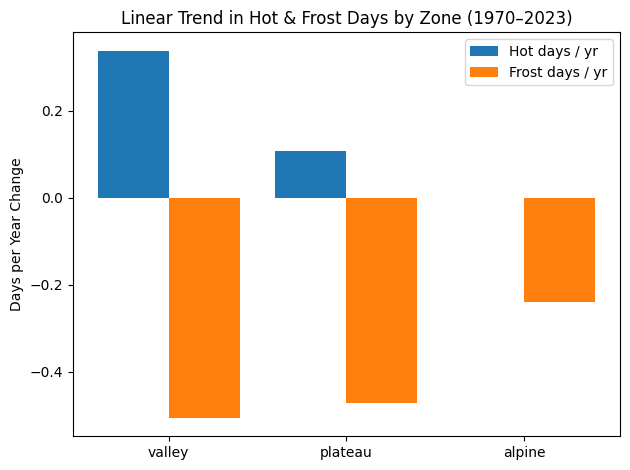
\includegraphics[width=0.45\textwidth]{img/linear_reg_trend.png}
  \caption{Estimated trend slopes in hot‐ and frost‐day counts (days per year) by zone.}
  \label{fig:linear_trend}
\end{figure}





\subsection{How do station installation dates and validity periods create spatio-temporal gaps, and where are the largest “data deserts”?}
\subsubsection{Objective}
The third research question investigates how the installation dates and operational periods of weather stations affect data availability over time and across Austrian regions and elevation zones. The goal is to identify spatial and temporal coverage gaps, also referred to as ``data deserts,'' that could affect the interpretation of long-term climate analyses.

\subsubsection{Methodology}

To address this question, the implementation proceeded in two main steps:

\begin{enumerate}
  \item \textbf{Metadata-Based Coverage Matrix:}  
    Using station metadata (installation and deactivation dates), a year-by-year activity matrix was constructed from 1960 to 2025 using a cross join. Active periods were filtered, and each station was assigned to one of five elevation bands:
    \begin{itemize}
      \item 0--499\,m (Lowland)
      \item 500--999\,m (Upland)
      \item 1000--1499\,m (Lower Alps)
      \item 1500--1999\,m (Alpine)
      \item 2000+\,m (High Alpine)
    \end{itemize}
    Aggregated counts by year, elevation zone, and federal state provided a theoretical view of station coverage.

  \item \textbf{Real Measurement-Based Coverage:}  
    To verify actual data presence, the climate dataset was filtered to include only records with at least one valid measurement. These were grouped using the same schema as the metadata-based approach.
\end{enumerate}

To keep the report focused, only the Lower Alps zone is discussed in detail as it highlights key patterns.

\subsubsection{Results and Interpretation}

\paragraph{Figure~\ref{fig:coverage_meta_loweralps}: Metadata-Based Coverage (Lower Alps)}  
The heatmap shows that while Tyrol and Salzburg maintained a consistent network of 10--30 active stations yearly since the 1970s, regions like Lower Austria and Upper Austria exhibit almost no presence in this elevation zone. This confirms topographic disparities in historical climate monitoring.

\begin{figure}[ht]
  \centering
    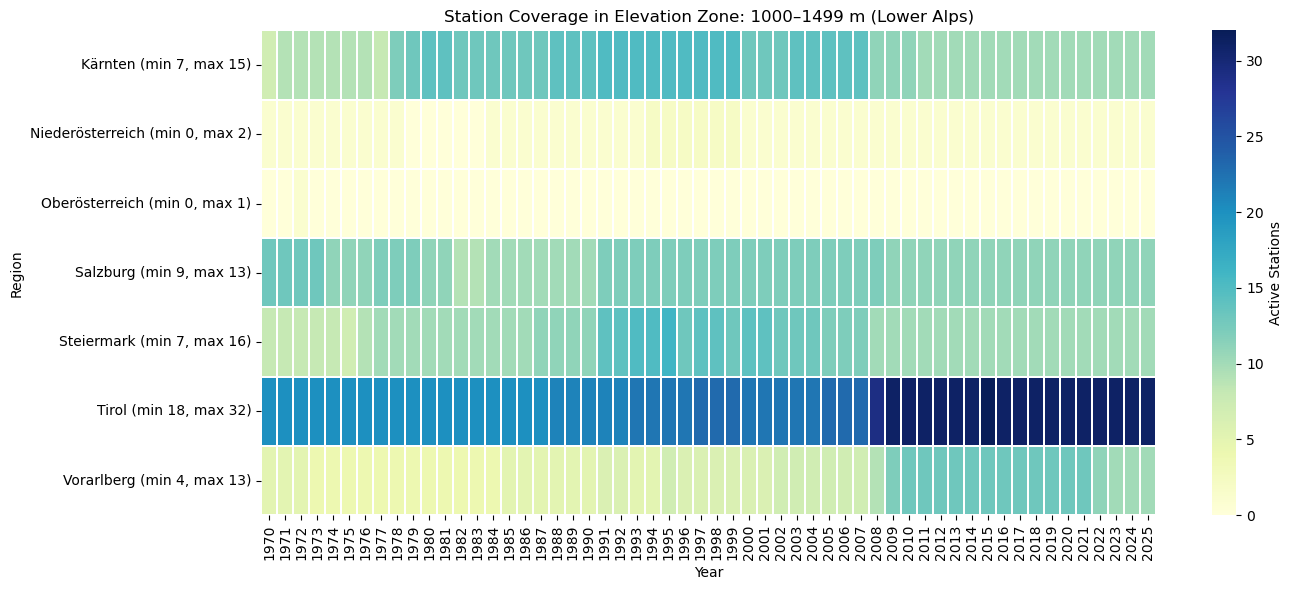
\includegraphics[width=0.45\textwidth]{img/coverage_zone_loweralps_meta.png}
    \caption{Metadata-based station coverage in elevation zone: 1000--1499\,m (Lower Alps)}
    \label{fig:coverage_meta_loweralps}
\end{figure}

\paragraph{Figure~\ref{fig:coverage_real_loweralps}: Actual Measurement-Based Coverage (Lower Alps)}  
The second heatmap confirms that actual measurement coverage aligns well with the metadata. Again, Tyrol is best represented, while several eastern federal states have minimal or no data-producing stations in this zone.

\begin{figure}[ht]
  \centering
    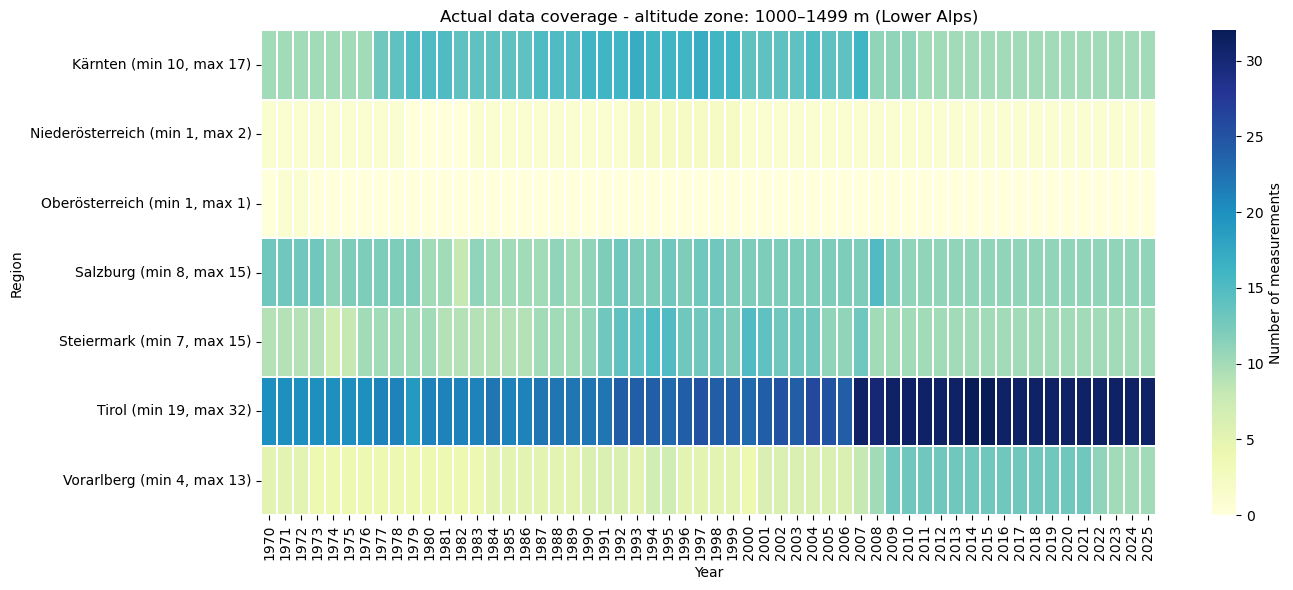
\includegraphics[width=0.45\textwidth]{img/data_coverage_loweralps.png}
    \caption{Actual measurement-based coverage in elevation zone: 1000--1499\,m (Lower Alps)}
    \label{fig:coverage_real_loweralps}
\end{figure}

\subsubsection{Conclusion}
Both metadata and actual measurement coverage confirm consistent long-term gaps in mid-altitude mountain zones across eastern Austrian regions. Western alpine states such as Tyrol provide dense and uninterrupted coverage. The stepwise implementation, beginning with metadata modeling and validated through real data filtering, proves effective in uncovering structural weaknesses in historical climate data availability.


\subsection{Which seasonal windows and locations optimize safety—combining sunshine hours, wind-gust flags, and frost/heat indicators?}
\subsubsection{Calculation Method}

The safety score is a composite metric designed to evaluate the environmental safety conditions for each weather station across Austria. It combines the following variables:

\begin{itemize}
    \item \textbf{Average Sunshine Hours}: Higher values are considered favorable.
    \item \textbf{Frequency of Wind Gusts}: Higher values are penalized due to increased hazard potential.
    \item \textbf{Frequency of Frost Days}: Higher values indicate harsher conditions and are penalized.
    \item \textbf{Frequency of Heat Days}: Moderately penalized to reflect discomfort and potential risk.
\end{itemize}

The score is calculated as a weighted sum:

\begin{equation}
\text{Score} = \text{Sunshine} - 2 \cdot \text{Wind Gust Freq} - 2 \cdot \text{Frost Freq} - 1.5 \cdot \text{Heat Freq}
\end{equation}

A higher safety score indicates more favorable and stable environmental conditions.

\subsubsection{Top Station Scores}

Table~\ref{tab:top_scores} shows the top 10 station-season combinations with the highest safety scores. These stations are located exclusively in high alpine zones (\textgreater 2000\,m) within Salzburg and exhibit high sunshine hours, but still significant wind and frost frequencies.

\begin{table}[H]
\centering
\begin{tabular}{|c|c|c|c|c|}
\hline
\textbf{Season} & \textbf{Station} & \textbf{Region} & \textbf{Sunshine [h]} & \textbf{Score} \\
\hline
Spring & 15410 & Salzburg & 461.3 & 398.8 \\
Spring & 213   & Salzburg & 440.8 & 378.2 \\
Spring & 15411 & Salzburg & 394.1 & 331.2 \\
Summer & 15410 & Salzburg & 336.1 & 291.5 \\
Spring & 15322 & Salzburg & 340.9 & 283.9 \\
Summer & 213   & Salzburg & 319.8 & 278.3 \\
Summer & 15411 & Salzburg & 279.7 & 243.9 \\
Winter & 15410 & Salzburg & 303.8 & 239.3 \\
Winter & 213   & Salzburg & 296.1 & 232.3 \\
Winter & 15411 & Salzburg & 294.0 & 231.4 \\
\hline
\end{tabular}
\caption{Top 10 Safety Scores by Station and Season}
\label{tab:top_scores}
\end{table}

\subsubsection{Visual Interpretation}

\begin{figure}[H]
    \centering
    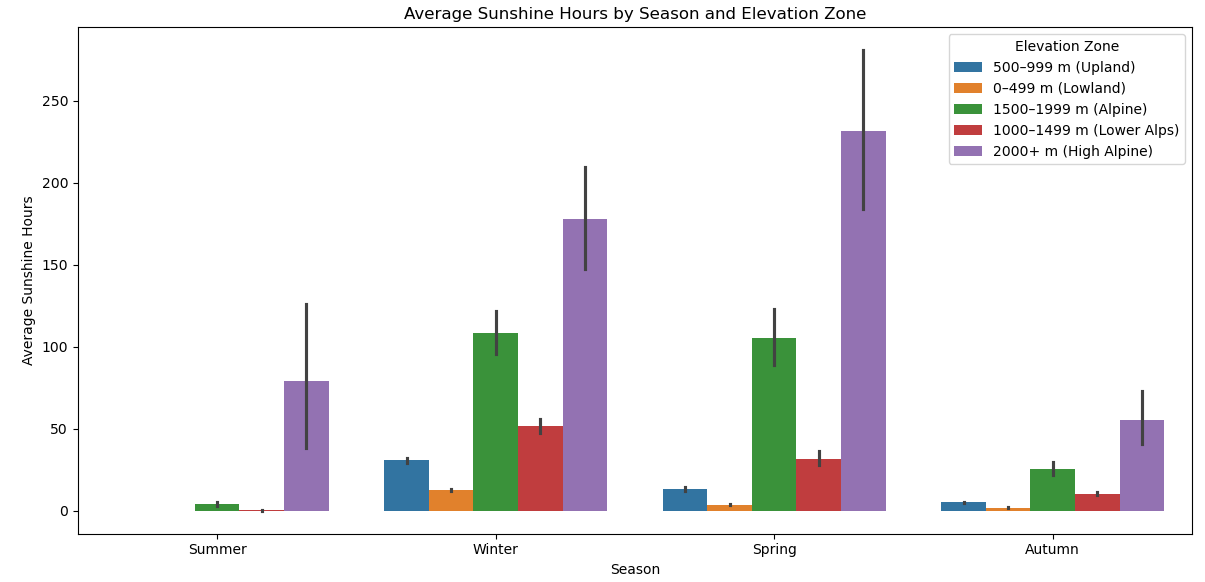
\includegraphics[width=0.45\textwidth]{img/sunshine_by_season_zone.png}
    \caption{Average Sunshine Hours by Season and Elevation Zone}
    \label{fig:sunshine}
\end{figure}

Figure~\ref{fig:sunshine} shows that the high alpine zone consistently records higher average sunshine hours across all seasons, especially in spring. This contributes positively to their safety scores.

\begin{figure}[H]
    \centering
    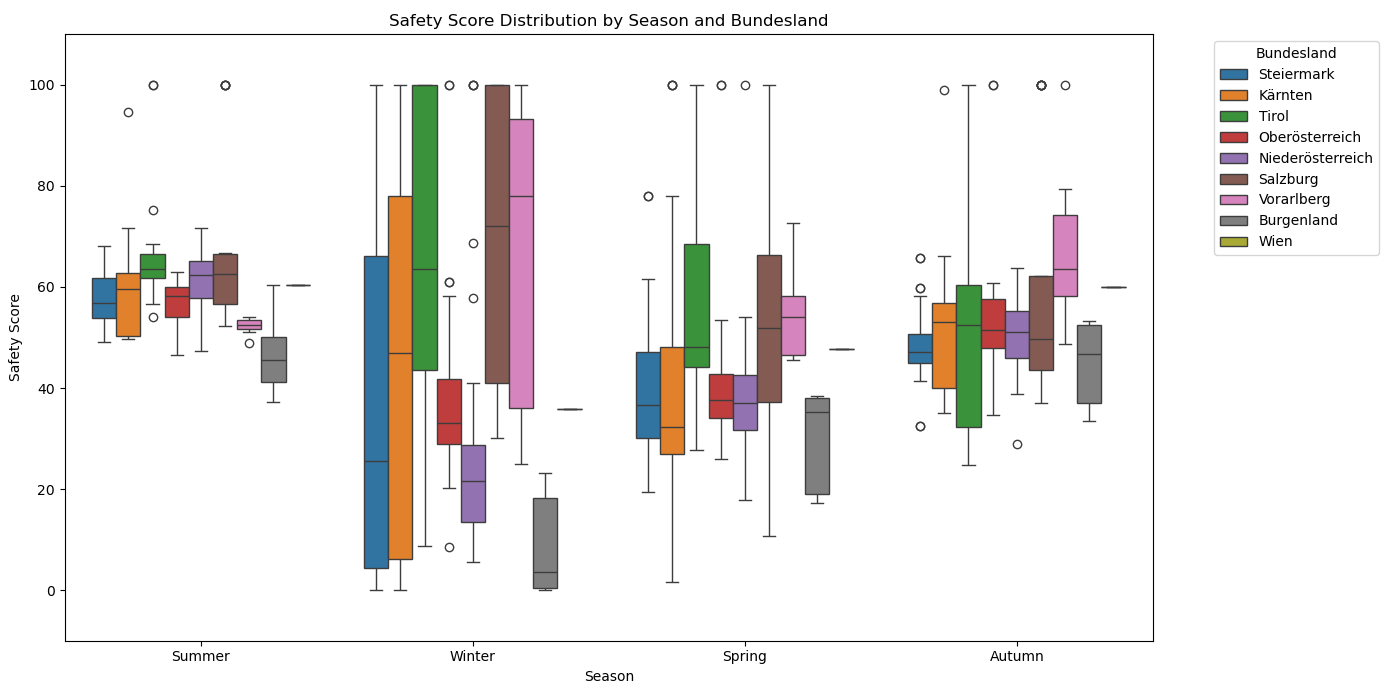
\includegraphics[width=0.45\textwidth]{img/safety_score_boxplot.png}
    \caption{Safety Score Distribution by Season and Bundesland}
    \label{fig:safety_boxplot}
\end{figure}

Figure~\ref{fig:safety_boxplot} presents the distribution of safety scores. Salzburg, Tirol, and Vorarlberg show the highest spread and highest values in winter and spring, corresponding to high-elevation stations.

\begin{figure}[H]
    \centering
    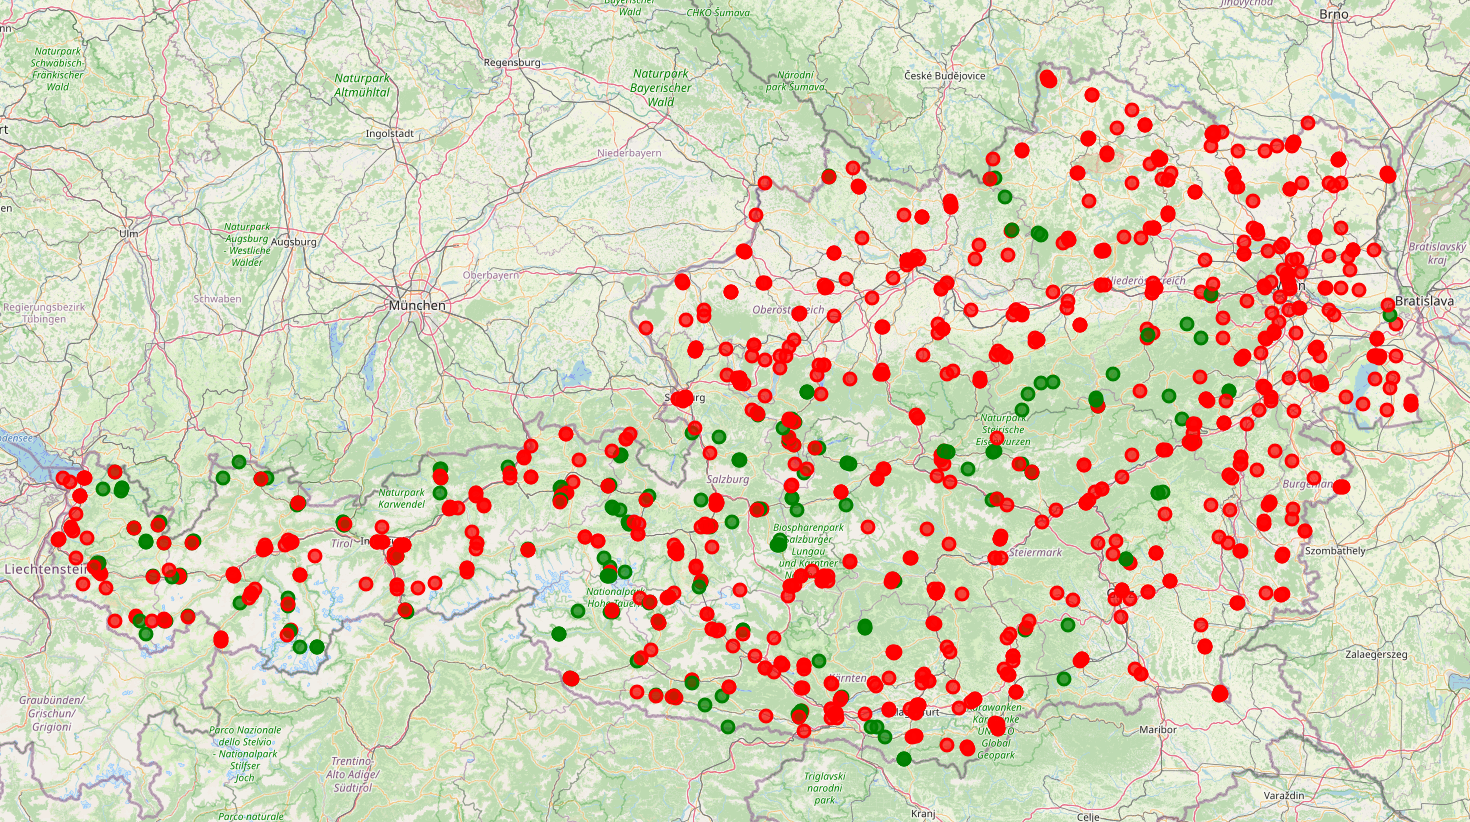
\includegraphics[width=0.45\textwidth]{img/station_map.png}
    \caption{Map of Stations by Safety Score (Green: High, Red: Low)}
    \label{fig:station_map}
\end{figure}

Figure~\ref{fig:station_map} visualizes the spatial distribution of safety scores. Green points indicate stations with relatively high safety scores, found predominantly in the Alpine regions. Red points represent stations with lower scores, more frequent in lower elevation areas.


\section{Conclusion}

\bibliographystyle{ACM-Reference-Format}
\bibliography{software}

\end{document}